\subsubsection{Atuadores}

% SLIDE DE ATUADORES
\begin{frame}
\frametitle{Atuadores}

O motor de passo foi escolhido para esse projeto devido a sua capacidade de realizar passos, que são rotações discretas incrementais e precisas. 

\begin{figure}
\centering
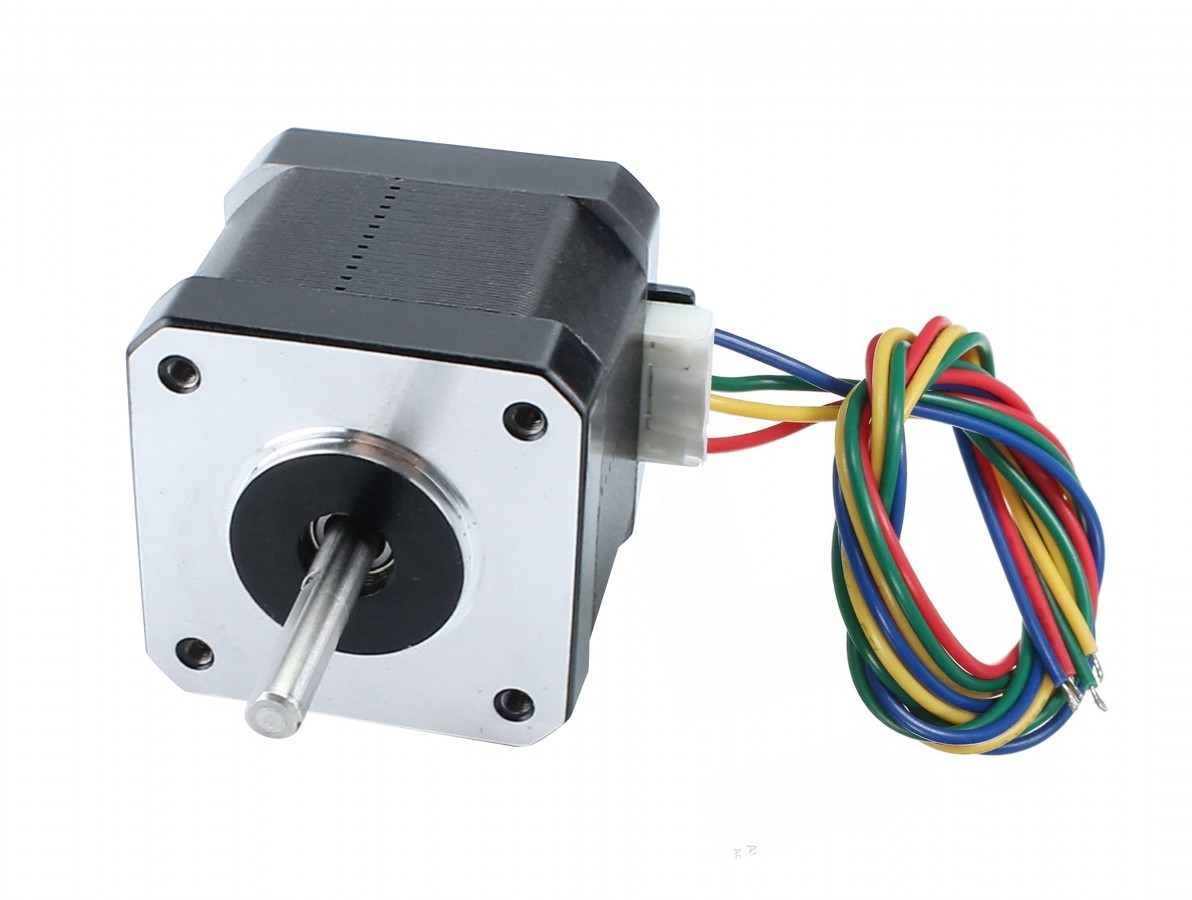
\includegraphics[scale = 0.1]{figs/motordepassoex}
\end{figure}

\end{frame}

% SLIDE DE ATUADORES
\begin{frame}
\frametitle{Atuadores}

Os passos são definidos por um número fixo de pólos magnéticos de dente de engrenagens do motor determinando assim, a precisão de ângulo de rotação do motor de passo.

\begin{figure}
\centering
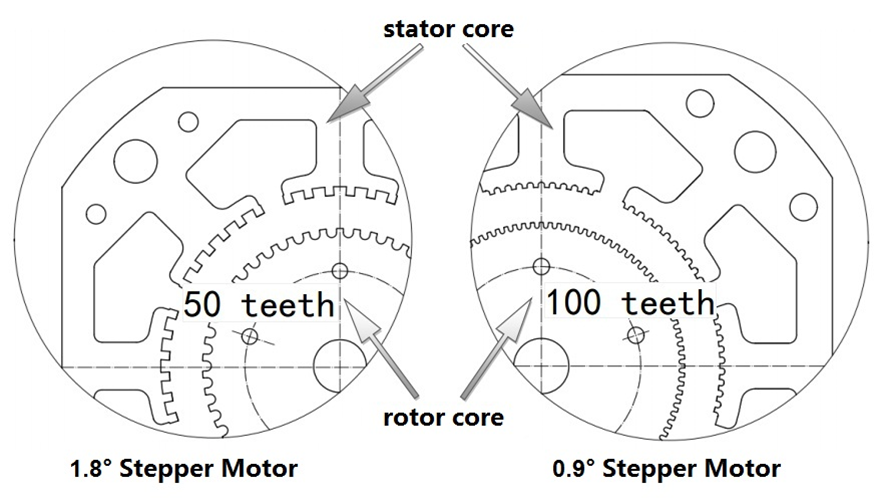
\includegraphics[scale = 0.3]{figs/didaticopasso}
\end{figure}

\end{frame}

% SLIDE DE ATUADORES
\begin{frame}
\frametitle{Atuadores}
\centering

\begin{figure}
\centering
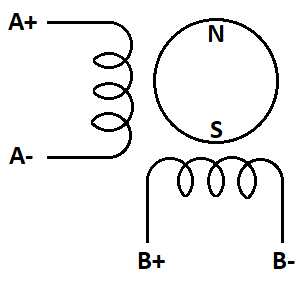
\includegraphics[scale = 0.5]{figs/meumotorbipolar}
\end{figure}
    
\begin{tabular}{cccccc}
    \hline
    \textbf{Passo} & \textbf{A+} & \textbf{B+} & \textbf{A-} & \textbf{B-} & \textbf{Decimal}\\
    \hline
    1 & 0 & 0 & 0 & 1 & 1\\
    2 & 0 & 0 & 1 & 0 & 2\\
    3 & 0 & 1 & 0 & 0 & 4\\
    4 & 1 & 0 & 0 & 0 & 8\\        
    \hline       
\end{tabular}
\end{frame}
